\documentclass[notes]{subfiles}

\begin{document}
	\chapter{Integrals}
	\addcontentsline{toc}{section}{4.1 - Areas \& Distances}
	\setcounter{section}{1}
	\fancyhead[RO,LE]{\bfseries \large\nameref{cs41}} 
	\fancyhead[LO,RE]{\bfseries \currentname}
	\fancyfoot[C]{{}}
	\fancyfoot[RO,LE]{\large \thepage}	%Footer on Right \thepage is pagenumber
	\fancyfoot[LO,RE]{\large Chapter 4.1}

\section*{Areas \& Distances}\label{cs41}
	\subsection*{Before Class}
	\addcontentsline{toc}{subsection}{Before Class}
	\subsubsection*{The Area Problem}
	\addcontentsline{toc}{subsubsection}{The Area Problem}
		\begin{ex}
			  The function $y = x^2$ on the interval $[0,1]$ is graphed below.
			\begin{center}
				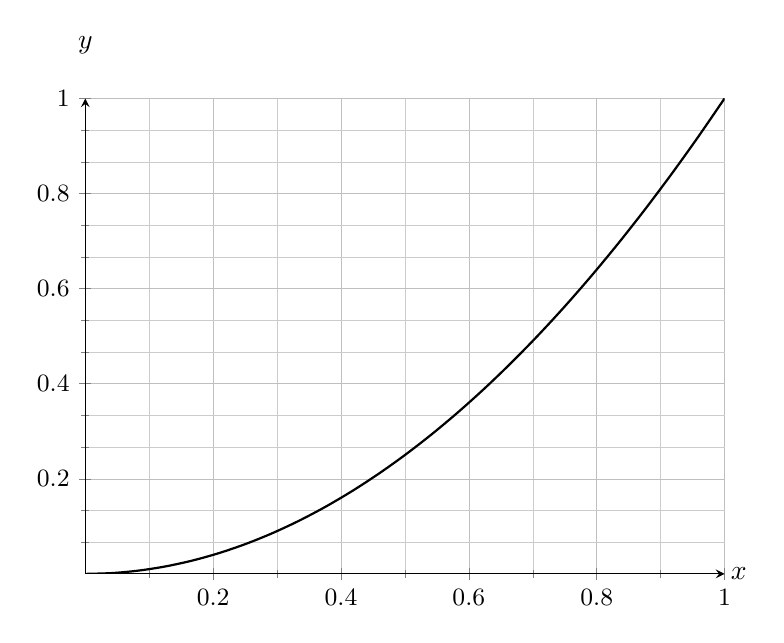
\begin{tikzpicture}
					\begin{axis}[
						height = 3in,
						width = .8\textwidth,
						grid = both,
						grid style={line width=.1pt, draw=gray!10},
						major grid style={line width=.2pt,draw=gray!50},
						minor grid style={line width=.2pt, draw=gray!40},
						every tick label/.append style={font=\small},
						axis x line = middle,
						axis y line = middle,
			    			every axis y label/.style={at={(ticklabel cs:1.15)}},
			    			%ytick = {-4, -2, -3, -1, 1, 2, 3, 4},
						y label style={at={(axis description cs:0,1.15)},anchor=north},
			    			ylabel = {$y$},
		    				every axis x label/.style= {at ={(ticklabel cs:1)}},
		    				%xtick = {-4,-3,-2,-1,1,2,3,4},
		    				x label style={at={(axis description cs:1.05,.0)},anchor=east},
		    				xlabel = {$x$},
		    				xmin = 0, xmax = 1,
		    				minor y tick num = 2,
		    				minor x tick num = 1
					]
					
						\addplot[thick, smooth, domain = 0:1] {x^2};
					\end{axis}
				\end{tikzpicture}
			\end{center}
		\begin{enumerate}[(a)]
			\item Use four rectangles to approximate the area under the parabola $y = x^2$ from 0 to 1; start from the left endpoint, 0.
				\vs{1}
				\newpage
				
			\item There are two ways of drawing the four rectangles$-$approximate the same area by starting with the right endpoint, 1.
				\vs{1}
		\end{enumerate}	
		\end{ex}	
			
		\begin{ex}
			Use eight rectangles to approximate the area under $y = x^2$ from 0 to 1, using both left and right endpoints.  Compare your estimates to the previous two calculations.
			\begin{flushleft}
				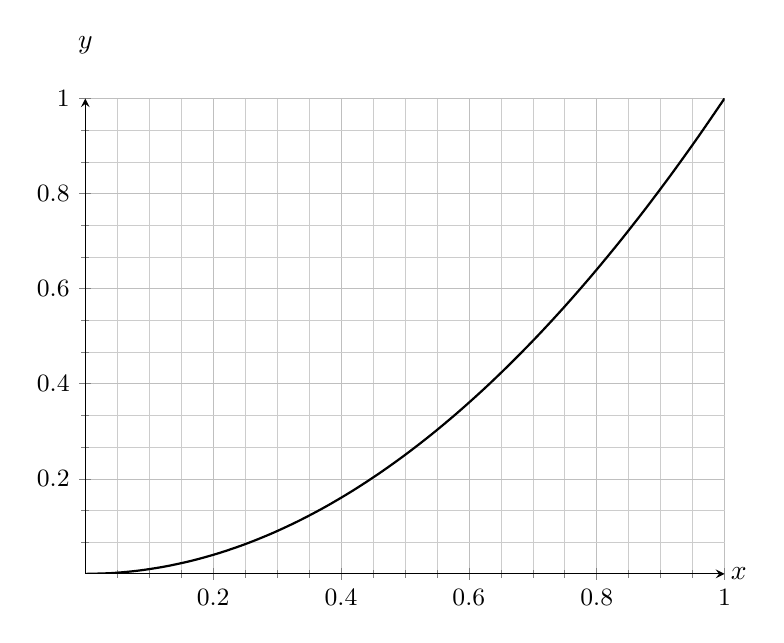
\begin{tikzpicture}
					\begin{axis}[
						height = 3in,
						width = .8\textwidth,
						every tick label/.append style={font=\small},
						axis x line = middle,
						axis y line = middle,
						grid = both,
						grid style={line width=.1pt, draw=gray!10},
						major grid style={line width=.2pt,draw=gray!50},
						minor grid style={line width=.2pt, draw=gray!40},
			    			every axis y label/.style={at={(ticklabel cs:1.15)}},
			    			%ytick = {-4, -2, -3, -1, 1, 2, 3, 4},
						y label style={at={(axis description cs:0,1.15)},anchor=north},
			    			ylabel = {$y$},
		    				every axis x label/.style= {at ={(ticklabel cs:1)}},
		    				%xtick = {-4,-3,-2,-1,1,2,3,4},
		    				x label style={at={(axis description cs:1.05,.0)},anchor=east},
		    				xlabel = {$x$},
		    				xmin = 0, xmax = 1,
		    				minor y tick num = 2,
		    				minor x tick num = 3
					]
					
						\addplot[thick, smooth, domain = 0:1] {x^2};
					\end{axis}
				\end{tikzpicture}
			\end{flushleft}
		\end{ex}
			\vs{3}
			
		\begin{question}
			What do you think would happen to our approximation of area if we used more rectangles?
		\end{question}
			\vs{.5}
			\newpage
		Generically, the process we are following has the following steps:
		\begin{rmk}[Approximating Area Under a Curve]
			\showto{ins}{
				\begin{enumerate}[(1)]
					\item Determine the length of the interval
					\item Subdivide into an $n$ equal subintervals
					\item For each subinterval, find the area of the approximating rectangle
					\item Sum the areas of the rectangles
				\end{enumerate}
			}
			\showto{st}{
				\begin{enumerate}[(1)]
				\setlength\itemsep{30pt}
					\item 
					\item 
					\item 
					\item 
				\end{enumerate}
			}
		\end{rmk}
		
		\begin{question}$ $
			\begin{enumerate}[(a)]
				\item If the interval we are concerned about is $[a,b]$, and we are using $n$ rectangles to approximate the area, how could we write the base length of each individual rectangle?  Denote the length by $\Delta x$.
					\vs{1}
					
				\item Let $a = x_0$.  How could we express $x_1$?  $x_2$?  What about a generic $x_i$, where $1\leq i\leq n$?
					\vs{1}
					
				\item Let $f(x_i)$ be the function value at $x_i$.  Using (a) and (b), write an expression for $S_n$, the sum of areas of our approximating rectangles.
					\vs{1}
			\end{enumerate}
		\end{question}
				\newpage
			
		\begin{rmk}[Left Rectangle Approximation]
			The left rectangle approximation for the area under the curve $f(x)$ on the interval $[a,b]$ (using $n$ rectangles) is given by
			\showto{ins}{
				\[L_n = f(x_0)\Delta x + f(x_1)\Delta x + \cdots + f(x_{n-2})\Delta x + f(x_{n-1})\Delta x\]
			}
			\showto{st}{
				\vspace{.75in} \\
			}
			or, in sigma notation,
			\showto{ins}{
				\[\sum_{i=0}^{n-1} f(x_i)\Delta x\]
			}
			\showto{st}{
				\\ \\ \\ \\
			}
			The $n$th left rectangle approximation is denoted $L_n$.
		\end{rmk}
			\vs{.25}

		\begin{rmk}[Right Rectangle Approximation]
			The right rectangle approximation for the area under the curve $f(x)$ on the interval $[a,b]$ (using $n$ rectangles) is given by
			\showto{ins}{
				\[R_n = f(x_1)\Delta x + f(x_2)\Delta x + \cdots + f(x_{n-1})\Delta x + f(x_n)\Delta x\]
			}
			\showto{st}{
				\vspace{.5in} \\
			}
			or, in sigma notation,
			\showto{ins}{
				\[\sum_{i=1}^{n} f(x_i)\Delta x\]
			}
			\showto{st}{
				\\ \\ \\ \\
			}
			The $n$th right rectangle approximation is denoted $R_n$.
		\end{rmk}
			\vs{.25}
		
	\subsubsection*{Sigma Notation}
	\addcontentsline{toc}{subsubsection}{Sigma Notation}
		\begin{rmk}[Sigma Notation]
			\emph{Sigma notation} is a shorthand way to write sums.  For example,
				\showto{ins}{\[\ds \sum_{i = 1}^n f(x_i) = f(x_0) + f(x_1) + f(x_2) + ... + f(x_{n-1}) + f(x_n)\]}
				\showto{st}{\\ \\ \\ \\ \\}
			Here, \showto{ins}{$i = 1$}\showto{st}{\blank{1}} refers to the \emph{starting index}, and \showto{ins}{$n$} \showto{st}{\blank{1}} is called the \emph{ending index}.  
		\end{rmk}	
		\newpage
		
		
	\subsubsection*{Pre-Class Activities}
	\addcontentsline{toc}{subsubsection}{Pre-Class Activities}
		\begin{ex}
			Consider $f(x) = \dfrac{1}{x}$.
			\begin{enumerate}[(a)]
				\item Carefully sketch the graph of $f(x)$ on the interval $[1,4]$.
					\vs{2.5}
					
				\item Find $R_3$, and draw the rectangles on your sketch.
					\vs{1}

				\item Express the sum from (b) in sigma notation.
					\vs{.5}
					
				\item Find $L_3$, and draw the rectangles on your sketch.
					\vs{1}
					
				\item Express the sum from (d) in sigma notation.
					\vs{.5}
					
			\end{enumerate}
		\end{ex}
			\newpage
			
		\begin{ex}
			Again, consider $f(x) = \dfrac{1}{x}$ on $[1,4]$.
			\begin{enumerate}[(a)]
				\item Resketch the graph of $f(x)$.
					\vs{1}
					
				\item Find $R_6$, and include the rectangles on your sketch from (a).  How do these rectangles compare to the $R_3$ rectangles?
					\vs{1}
					
				\item Find $L_6$, and include the rectangles on your sketch from (a).  How do these rectangles compare to the $L_3$ rectangles?
					\vs{1}
 
			\end{enumerate}
		\end{ex}
			\newpage
			
	\subsection*{In-Class}	
	\addcontentsline{toc}{subsection}{In-Class}
		\begin{ex}
			For $f(x) = x^2$ on $[0,1]$, show that the sum of the areas of the upper approximating rectangles approaches $\dfrac{1}{3}$, i.e. $\ds \lim_{n\to\infty} R_n = \dfrac{1}{3}$.
		\end{ex}
			\newpage
	
		\begin{defn}[Area Under a Curve]
			The \textbf{area} of the region $S$ that lies under the graph of the continuous function $f$ is the limit of the sum of the areas of approximating rectangles:
				\showto{ins}{
					\[A= \lim_{n\to \infty} R_n = \lim_{n\to\infty} \sum_{i=1}^n f(x_i)\Delta x\]
				}
				\showto{st}{\\
					\vspace{.5in}
				}
				or
				\showto{ins}{
					\[A= \lim_{n\to \infty} L_n = \lim_{n\to\infty} \sum_{i=0}^{n-1} f(x_i)\Delta x\]
				}
				\showto{st}{
					\vspace{.5in}
				}
		\end{defn}
			
		\begin{ex}
			Let $A$ be the area of the region that lies under the graph of $f(x) = x^3$ between $x = 1$ and $x = b$, where $1\leq b\leq 3$.
			\begin{enumerate}[(a)]
				\item Using left endpoints, find an expression for $A$ as a limit; do not evaluate the limit.
					\vs{1}
				\item Estimate the area when $b = 3$ by using four subintervals.
					\vs{1}
			\end{enumerate}
		\end{ex}
		
		\begin{ex}
			The expression $\ds \lim_{n\to \infty} \sum_{i=1}^n \dfrac{3}{n} \sqrt{1+\dfrac{3i}{n}}$ gives the area of a region; describe such a region.  \emph{Do not try to evaluate the limit}.
		\end{ex}
			\vs{1}
			
			\newpage
		
	\subsubsection*{The Distance Problem}
	\addcontentsline{toc}{subsubsection}{The Distance Problem}
		Given constant velocity, we can use the formula $\text{distance} = \text{velocity }\times \text{ time}$ to calculate the distance an object travels over a certain period of time.  
		\begin{ex}
			Consider a moving car, with increasing velocity.  The velocity was measured every two seconds, and the results collected in the table below.
			\begin{center}
				{\renewcommand{\arraystretch}{1.2}
				\begin{tabular}{|c|c|c|c|c|c|c|} \hline
					Time (sec) & 0 & 2 & 4 & 6 & 8 & 10 \\ \hline
					Velocity (ft/sec) & 20 & 30 & 38 & 44 & 48 & 50 \\ \hline
				\end{tabular}
				}
			\end{center}
		\begin{enumerate}[(a)]
			\item Find an upper estimate for the distance the car traveled in 10 seconds.
				\vs{1}
				
			\item Find a lower estimate for the distance the car traveled in 10 seconds.
				\vs{1}
				
		\end{enumerate}
		\end{ex}	
			
		\begin{ex}
			Roger is training for a marathon.  His friend Jeff rides behind him on a bicycle and clocks his speed every 15 minutes.  Roger starts out strong, but stops after an hour and a half.  
			\begin{center}
				{\renewcommand{\arraystretch}{1.2}
				\begin{tabular}{|c|c|c|c|c|c|c|c|} \hline
					Time elapsed (min) & 0 & 15 & 30 & 45 & 60 & 75 & 90 \\ \hline
					Speed (mph) & 12 & 11 & 10 & 10 & 8 & 7 & 0 \\ \hline
				\end{tabular}
				}
			\end{center}
			Give upper and lower rectangle estimates for the distance Roger ran.
		\end{ex}
			\vs{1}
			\newpage
			
	\subsection*{After Class}
	\addcontentsline{toc}{subsection}{After Class}
		\begin{ex}
			We showed that, for $f(x) = x^2$ on $[0,1]$, $\ds \lim_{n\to \infty} R_n = \dfrac{1}{3}$ was the area under the curve.  Show that $\ds \lim_{n\to \infty} L_n = \dfrac{1}{3}$ as well.  Use the fact that $\ds \sum_{i=1}^n f(x_i)\Delta x = \sum_{i=0}^{n-1} f(x_{i+1})\Delta x$ and that $\ds \sum_{i=1}^n i =\dfrac{n(n+1)}{2}$
		\end{ex}
			\vs{2}
			
		\begin{ex}
			A stock car prototype is being tested.  Over the course of one minute, its speed was recorded in ten second intervals.
			\begin{center}
				{\renewcommand{\arraystretch}{1.2}
				\begin{tabular}{|c|c|c|c|c|c|c|c|} \hline
					Time (sec) & 0 & 10 & 20 & 30 & 40 & 50 & 60 \\ \hline
					Velocity (mi/h) & 182.9 & 168 & 106.6 & 99.8 & 124.5 & 176.1 & 175.6\\ \hline
				\end{tabular}
				}
			\end{center}
			Find upper and lower estimates for the distance traveled by the car in one minute.
		\end{ex}
			\vs{1}
			\newpage
			
		\begin{ex}
			If a curve measures the rate of change of some function, what is the \emph{explicit connection} between the area under the curve on a given interval and the total change of the function on that interval?
		\end{ex}
			\vs{1}
	\clearpage
\end{document}